\documentclass{beamer}
\usepackage[latin1]{inputenc}
\usepackage{amsmath}
\usepackage{graphicx}
\usepackage{multimedia}
\usepackage{caption}
\usetheme{default}
\usecolortheme{default}
\definecolor{darkred}{RGB}{24,0,0}
\setbeamercolor{title}{fg=red}
%\setbeamercolor{frametitle}{fg=black}
\setbeamertemplate{blocks}[rounded][shadow=true]
\setbeamertemplate{itemize items}[square]
\usefonttheme{serif}
\title{\textit{\textbf{The effect of gas bulk rotation on the morphology of the Ly$\alpha$ line.}}}
\author{Juan Nicol\'as Garavito-Camargo \\ Advisor: Jaime E. Forero-Romero}
\institute{Universidad de los Andes, Bogot\'a, Colombia}
\date{May 20, 2015}
\begin{document}

\begin{frame}
\titlepage
\author
\institute
\begin{figure}
%\rule{1.28cm}{0.72cm}

\includegraphics[scale=0.35]{Figures/logo.jpeg}
\end{figure}
\textit{\textbf{In collaboration with Mark Dijkstra.}}
\end{frame}

\begin{frame}{\textit{\textbf{Emission lines: Transitions from higher to lower energy levels in the atoms.}}}
\begin{figure}
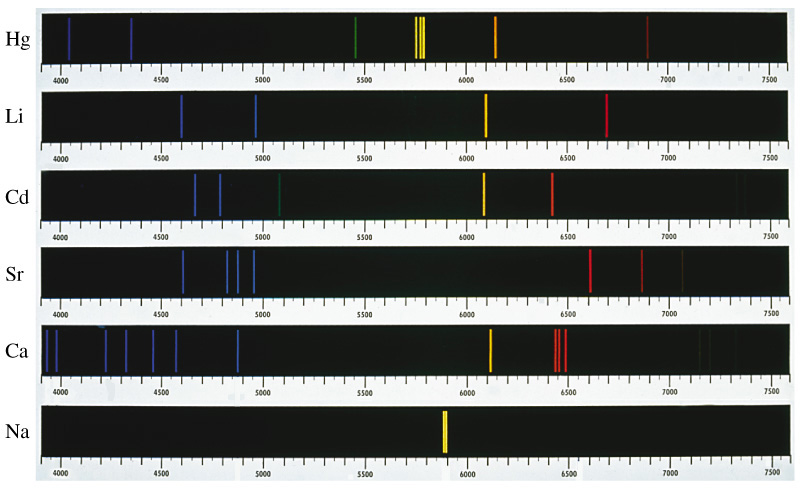
\includegraphics[scale=0.35]{Figures/emission.jpg}
\caption*{Wavelenght($\AA$)}
\end{figure}
\end{frame}

\begin{frame}{\textit{\textbf{Hydrogen is the most abundant element in the Universe.}}}
\begin{figure}
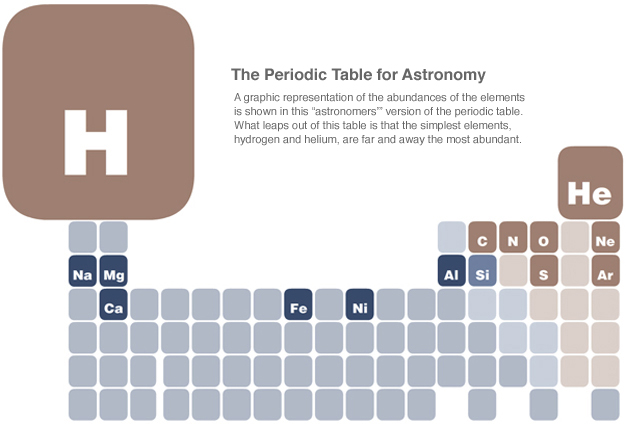
\includegraphics[scale=0.3]{Figures/astronomy_table.jpg}
\caption{Astronomers periodic table. Image credit: http://chandra.harvard.edu}
\end{figure}
\end{frame}



\begin{frame}{\textit{\textbf{The Lyman $\alpha$ emission line is the transition from the first state to the ground state in the Hydrogen atom.}}}
A Ly$\alpha$ photon is emitted with a $\lambda= 121.56 nm$.
\begin{figure}
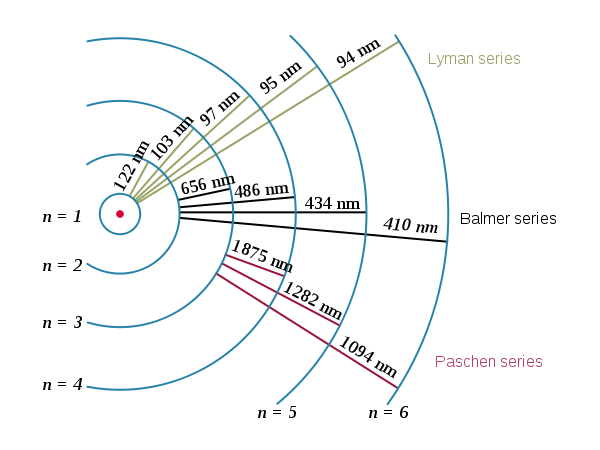
\includegraphics[scale=0.4]{Figures/Hydrogen_transitions.png}
\end{figure}
\end{frame}

\begin{frame}{\textit{\textbf{Ly$\alpha$ is in the UV part of the EM spectrum.}}}
\begin{figure}
\centering
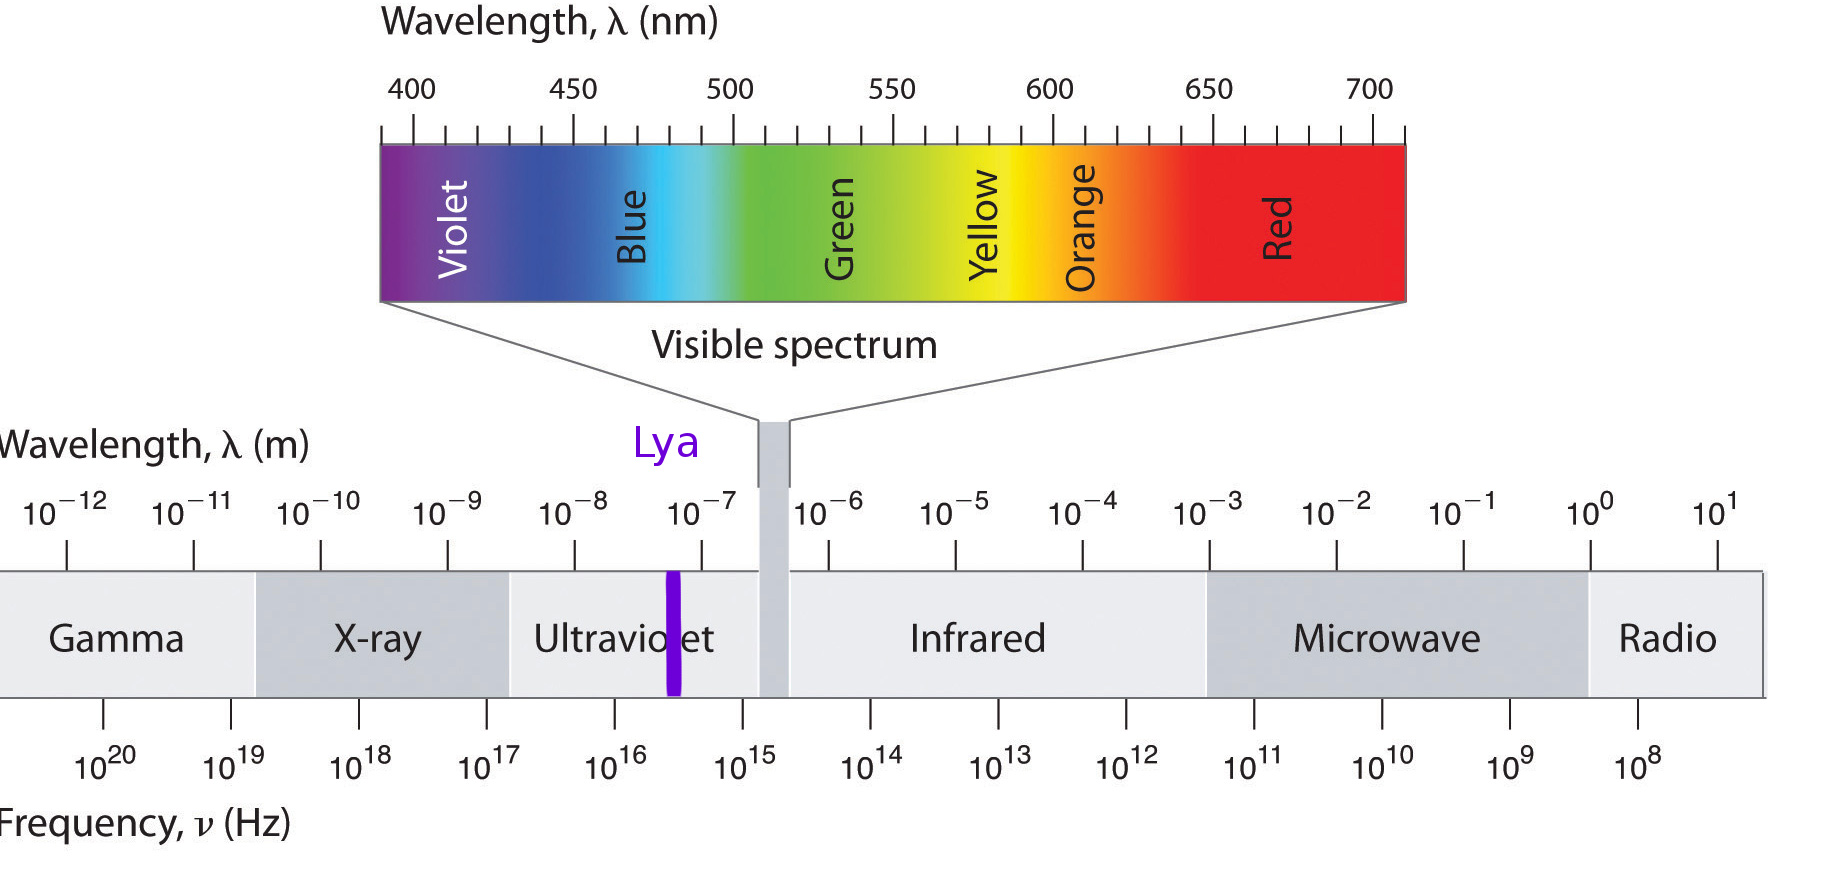
\includegraphics[scale=0.18]{Figures/em.jpg}
\end{figure}
\end{frame}


\begin{frame}{\textit{\textbf{The Ly $\alpha$ is no observable from earth.}}}
\begin{figure}
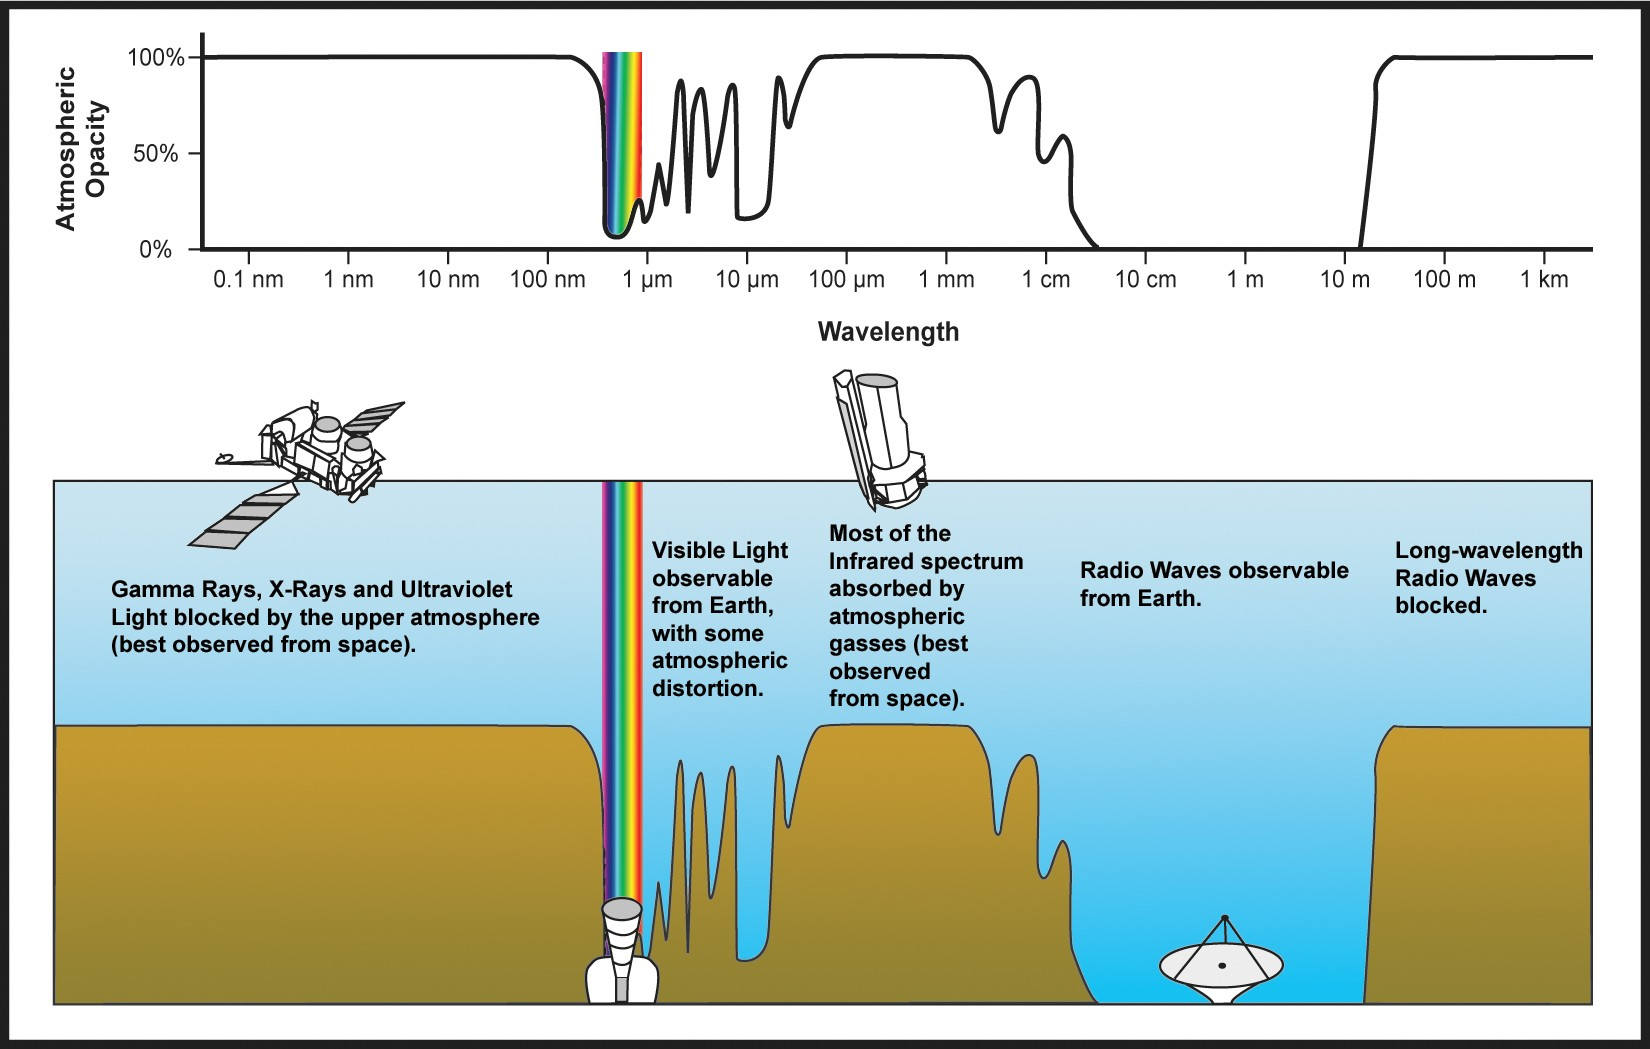
\includegraphics[scale=0.8]{Figures/AtmosphericEM.jpg}
\caption*{Atmospheric radiation absorption}
\end{figure}
\end{frame}


%\begin{frame}
%Lya line characteristics
%\end{frame}

\begin{frame}{\textit{\textbf{Due to the cosmological redshift LAEs are visibles from earth.}}}
\begin{figure}
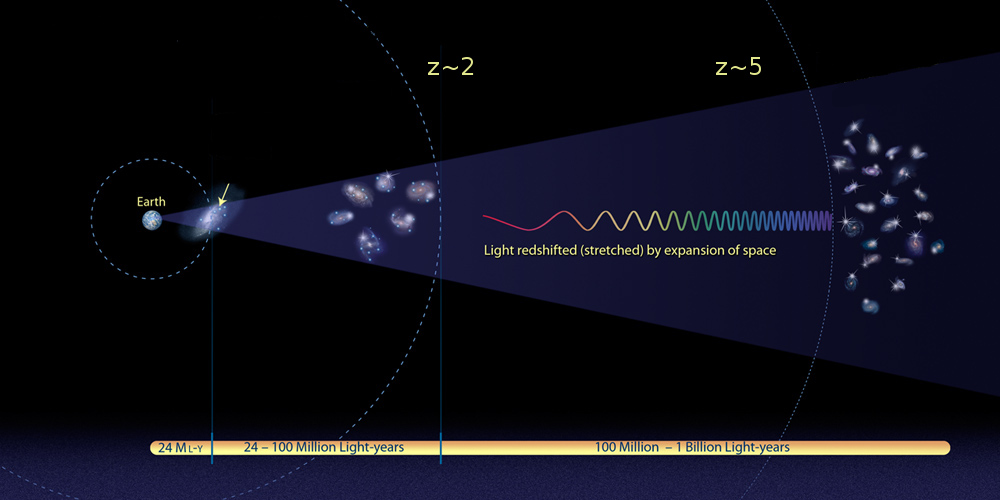
\includegraphics[scale=0.3]{Figures/expansion.jpg}
\caption*{Image credit: NASA, ESA, and A. Feild (STScI).}
\end{figure}
\end{frame}

\begin{frame}
\begin{center}
\LARGE{ How galaxies radiate Ly$\alpha$ photons:}
\end{center}
\end{frame}


\begin{frame}{\textit{\textbf{UV radiation mechanisms and sources:}}}

\textbf{1. UV stellar radiation.} \\ 
\begin{figure}
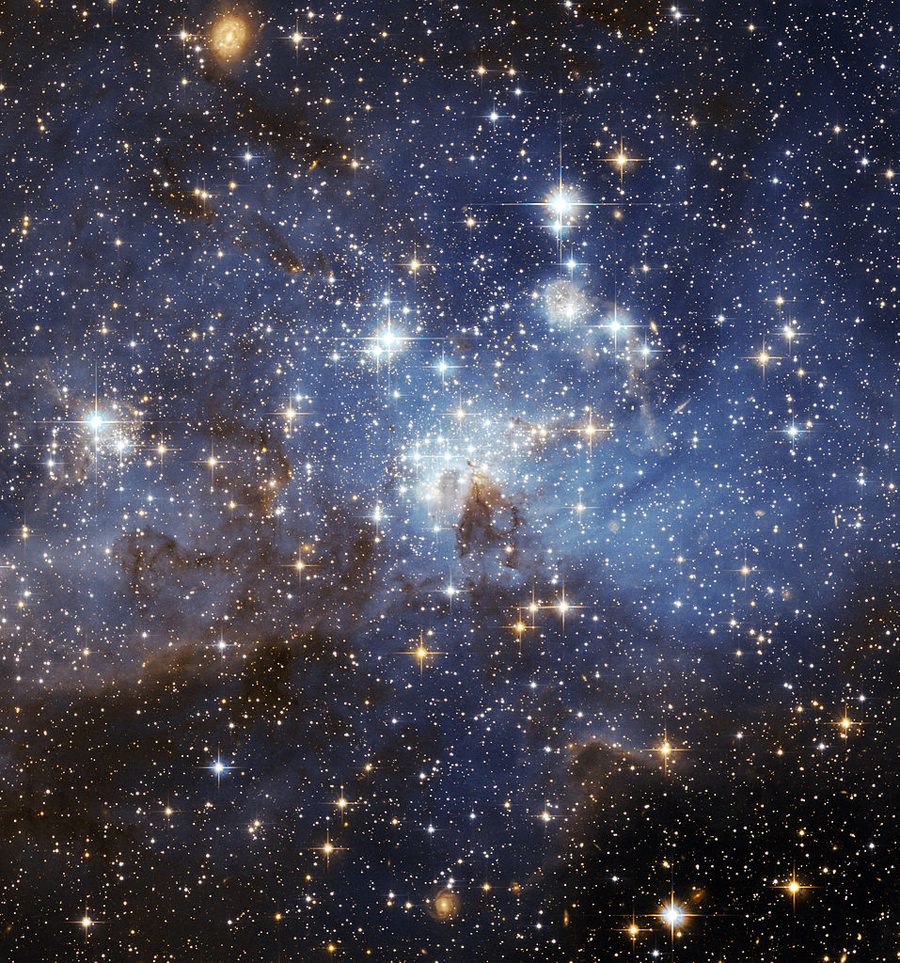
\includegraphics[scale=0.2]{Figures/stars.jpg}
\end{figure}
\end{frame}


\begin{frame}{Gravitational cooling \& UV background radiation:}
\begin{figure}
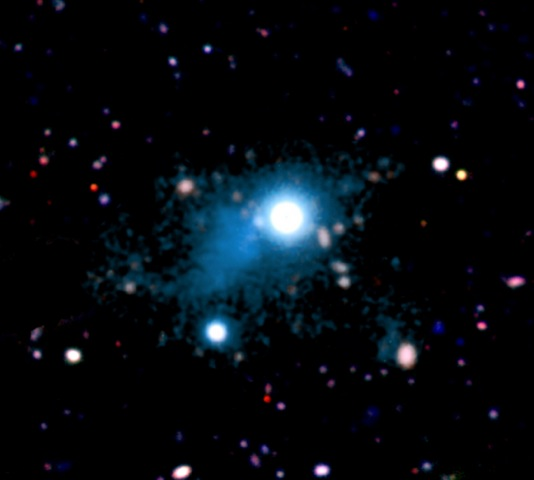
\includegraphics[scale=0.4]{Figures/quasar.jpg}
\caption*{Cantalupo, e.a. MNRAS 2012}
\end{figure}
\end{frame}

\begin{frame}%n{figure}
\begin{figure}
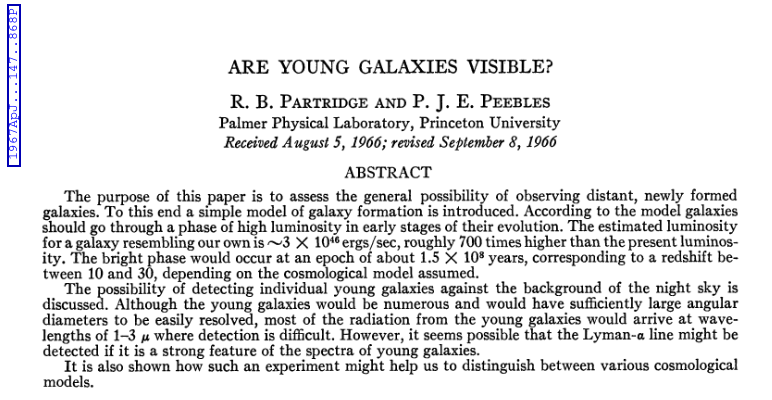
\includegraphics[scale=0.4]{Figures/PP.png}
\end{figure}
\end{frame}


\begin{frame}
\LARGE{25 years later ...}
\end{frame}

\begin{frame}
\begin{figure}
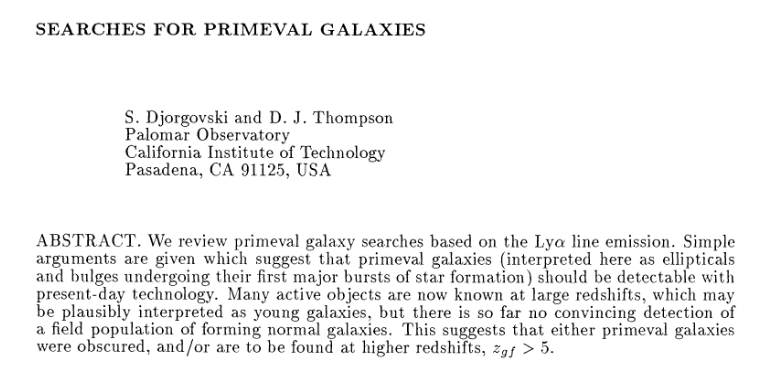
\includegraphics[scale=0.4]{Figures/DJT.png}
\end{figure}
\end{frame}

\begin{frame}%{Ly $\alpha$ as an important tool in extragalactic astronomy}
\begin{figure}
\begin{flalign*}
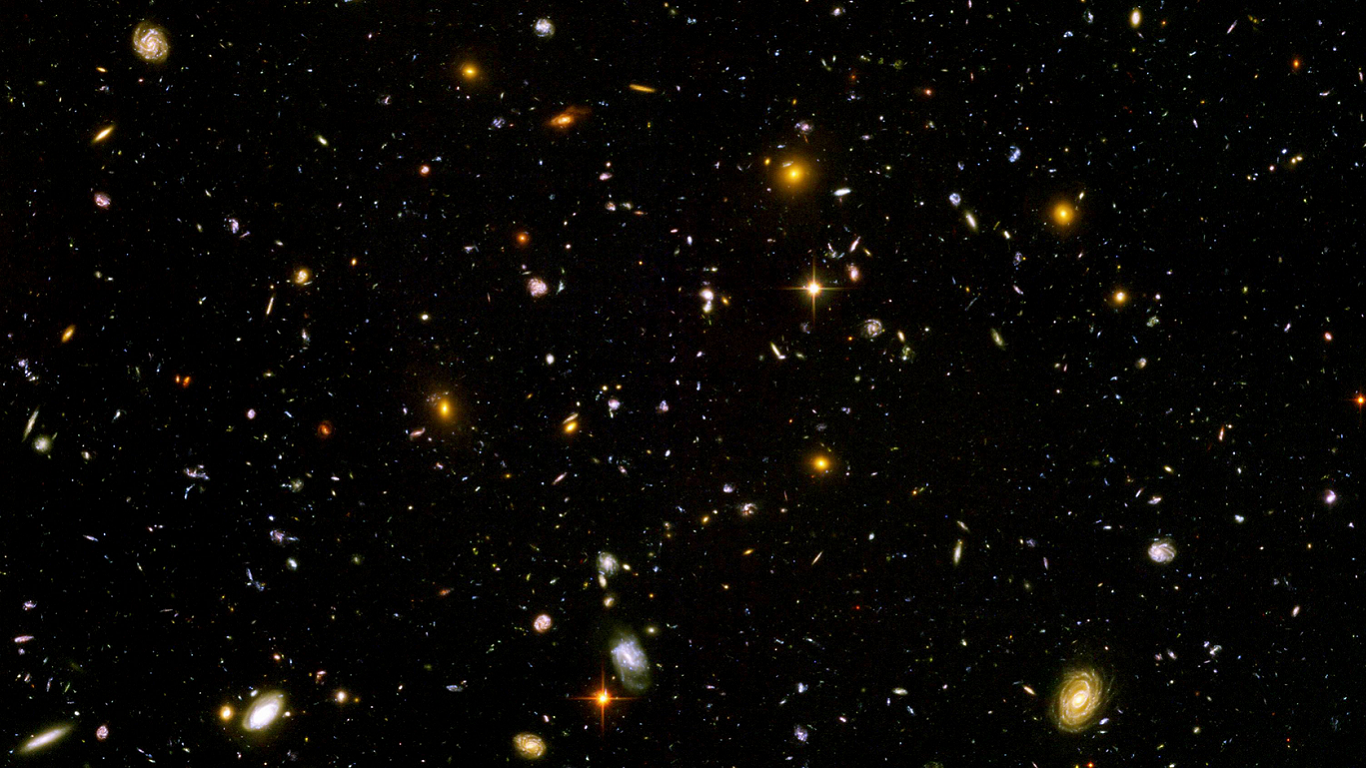
\includegraphics[scale=0.3]{Figures/hdf.png}
\end{flalign*}
\caption*{Hubble deep field.}
\end{figure}
\end{frame}

% units convention 
\begin{frame}{Units convention:}
\[
x = \dfrac{\nu_{obs} - \nu_{\alpha}}{\Delta \nu_{D}} 
\]

\[
\Delta \nu_{D} = \dfrac{v_{th}}{c}\nu_{\alpha}
\]

\[
V = x v_{th} = \dfrac{(\nu_{obs} - \nu_{\alpha})}{\nu_{\alpha}} c
\]

\end{frame}

\begin{frame}{\textit{\textbf{LAEs spectra are diverse:}}}
\begin{figure}
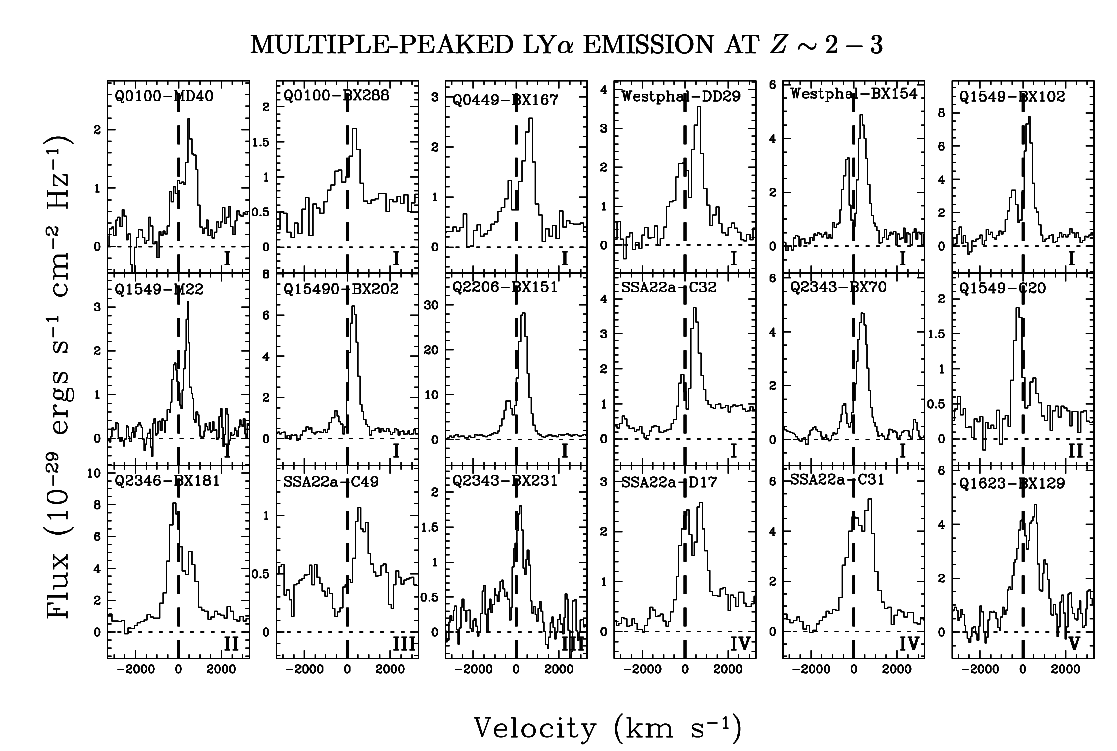
\includegraphics[scale=0.27]{Figures/kulas.png}
\caption*{Kulas e.a ApJ, 2012.}
\end{figure}
\end{frame}

\begin{frame}{\textit{\textbf{Radiative transfer is more complex than usual:}}}
\begin{figure}
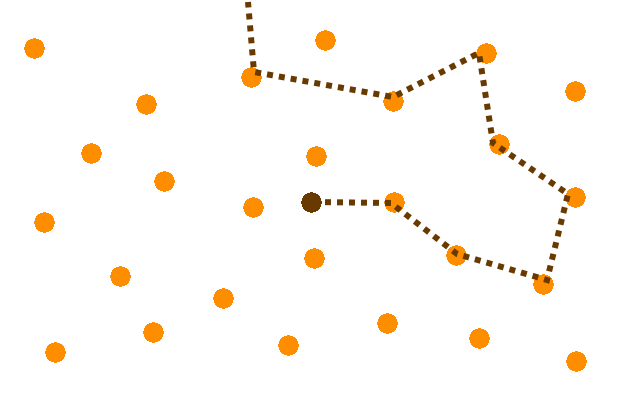
\includegraphics[scale=0.3]{Figures/RT.png}
\end{figure}
\end{frame}

\begin{frame}{\textit{\textbf{Radiative transfer in a non-static medium induces	 shifts on the line:}}}
\begin{figure}
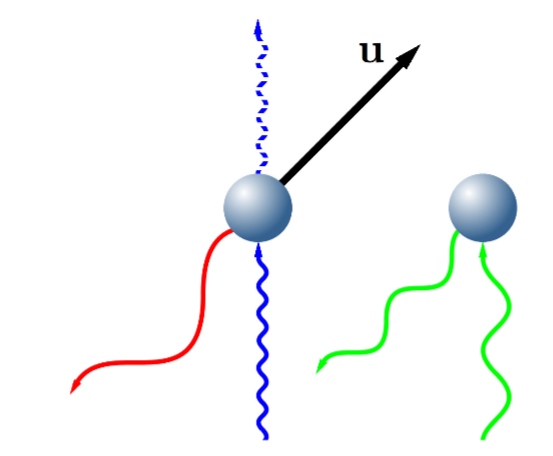
\includegraphics[scale=0.4]{Figures/xshift.png}
\caption*{Laursen, P. PhDT, 2010.}
\end{figure}
\end{frame}


\begin{frame}{\textit{\textbf{Ly$\alpha$ line is shaped by density, temperature and velocity}}}
\begin{figure}
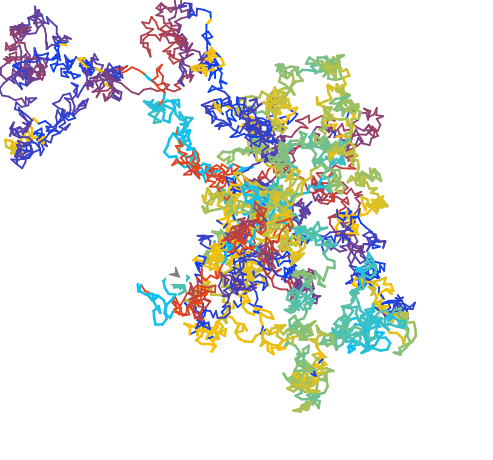
\includegraphics[scale=0.4]{Figures/rand_walk.png}
\end{figure}
\end{frame}

\begin{frame}{\textit{\textbf{Dust absorbs Ly$\alpha$ photons}}}
Dust grains can either absorbe or scatter Ly$\alpha$ photons. The probability
of these events is given by the \textbf{Albedo (A)}.

\[   
A = \dfrac{\sigma_{scatt}}{\sigma_{dust}}
\]

 
\end{frame}

\begin{frame}{\textit{\textbf{Optical depth:}}}
\LARGE{$\tau = nL\sigma$}
\begin{figure}
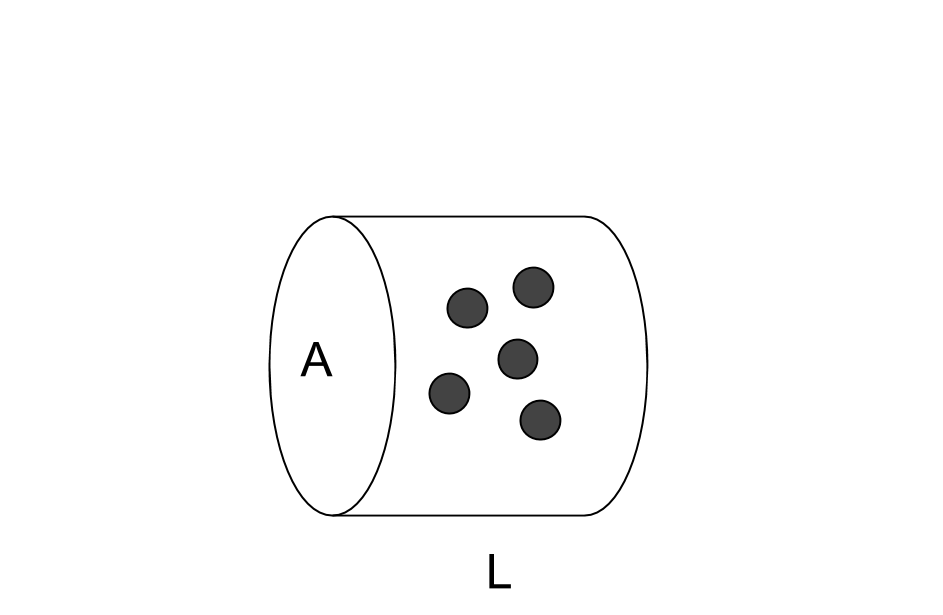
\includegraphics[scale=0.3]{Figures/od.png}
\end{figure} 
\end{frame}


\begin{frame}{\textit{\textbf{Radiative transfer as diffusion process:}}}

\begin{equation}\label{eq:analytic}
\dfrac{d J(\nu)}{d\tau} = \dfrac{(\Delta \nu_D)^2}{2}\dfrac{\partial}{\partial \nu}\phi (\nu) \dfrac{\partial J(\nu)}{\partial \nu}
\end{equation}

Where $\nu$ is the frequency of the photons, $\phi(\nu)$ is the Voigt profile and $\tau$
the optical depth.

\begin{figure}
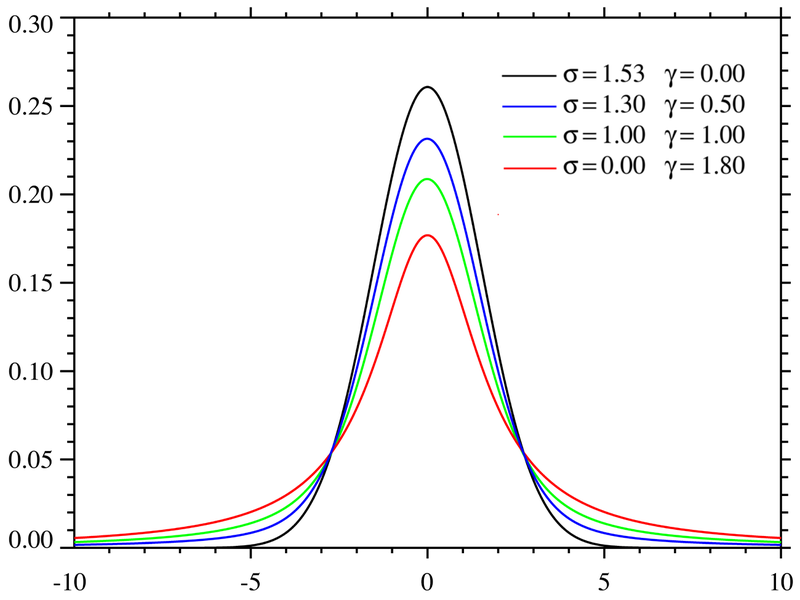
\includegraphics[scale=0.2]{Figures/voigt.png}
\caption{Voigt profile}
\end{figure}

\end{frame}



\begin{frame}{\textit{\textbf{A slab geometry induces a double-peak in the line:}}}
\begin{figure}
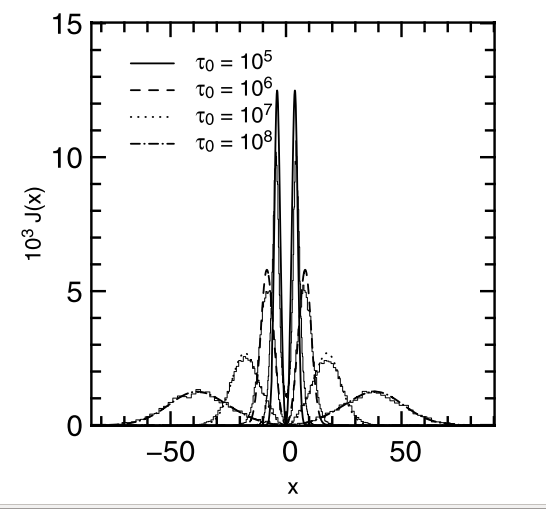
\includegraphics[scale=0.4]{Figures/slab.png}
\caption*{Forero-Romero e.a 2011.}
\end{figure}
\end{frame}


\begin{frame}{\textit{\textbf{A spherical distribution induces a double-peak in the line:}}}
\begin{figure}
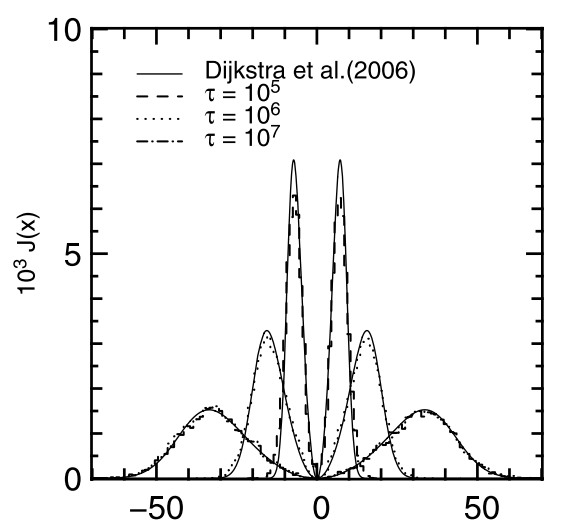
\includegraphics[scale=0.35]{Figures/sphere.png}
\caption*{Forero-Romero e.a 2011.}
\end{figure}
\end{frame}
%-------------------------- Previous studies ---------------------

\begin{frame}
\LARGE{Monte-Carlo approach:}
\end{frame}

\begin{frame}{\textit{\textbf{Radiative Transfer via Monte-Carlo methods:}}}
\begin{figure}
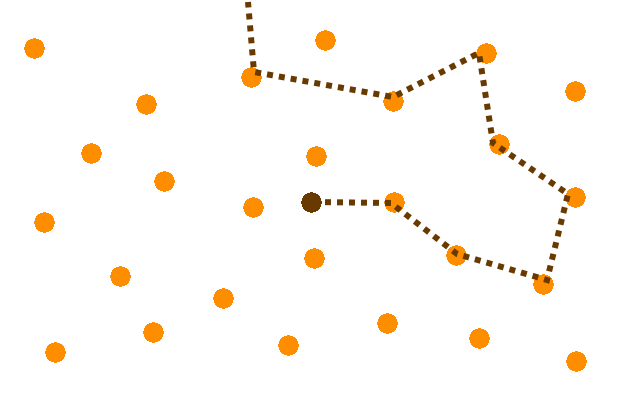
\includegraphics[scale=0.3]{Figures/RT.png}
\end{figure}
\end{frame}



\begin{frame}{\textit{\textbf{Asymmetries in the line can be induced by kinematics:}}}
\begin{figure}
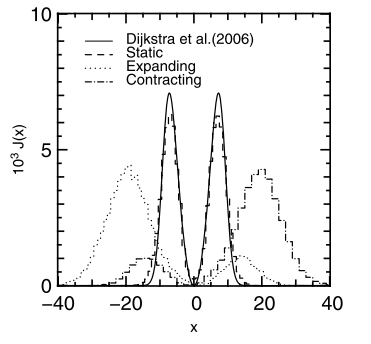
\includegraphics[scale=0.5]{Figures/expanding.png}
\caption*{Forero-Romero e.a 2011.}
\end{figure}
\end{frame}




%\begin{frame}{Cavities}
%Zheng/Zheng and Dijkstra
%\end{frame}

\begin{frame}{\textit{\textbf{Thin shell model:}}}
\begin{figure}
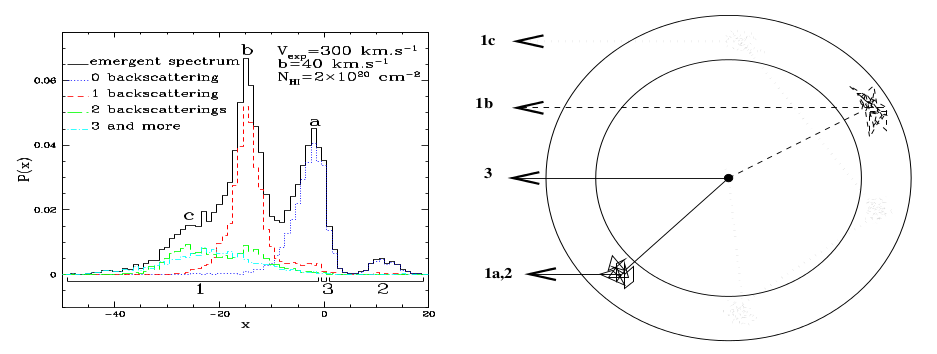
\includegraphics[scale=0.3]{Figures/shell.png}
\caption*{Verhamme, A. e.a, A\&A, 2006.}
\end{figure}
\end{frame}

\begin{frame}
\LARGE{Different geometries and kinematics of the gas has an impact on the morphology of the
Ly$\alpha$ spectrum.}\\

\end{frame}


%---------------------RESULTS-----------------------------

\begin{frame}
\LARGE{What would be the effect of rotation on the morphology of the Ly$\alpha$ line?\\ 
Is this effect observable?} 
\end{frame}


\begin{frame}
\begin{figure}
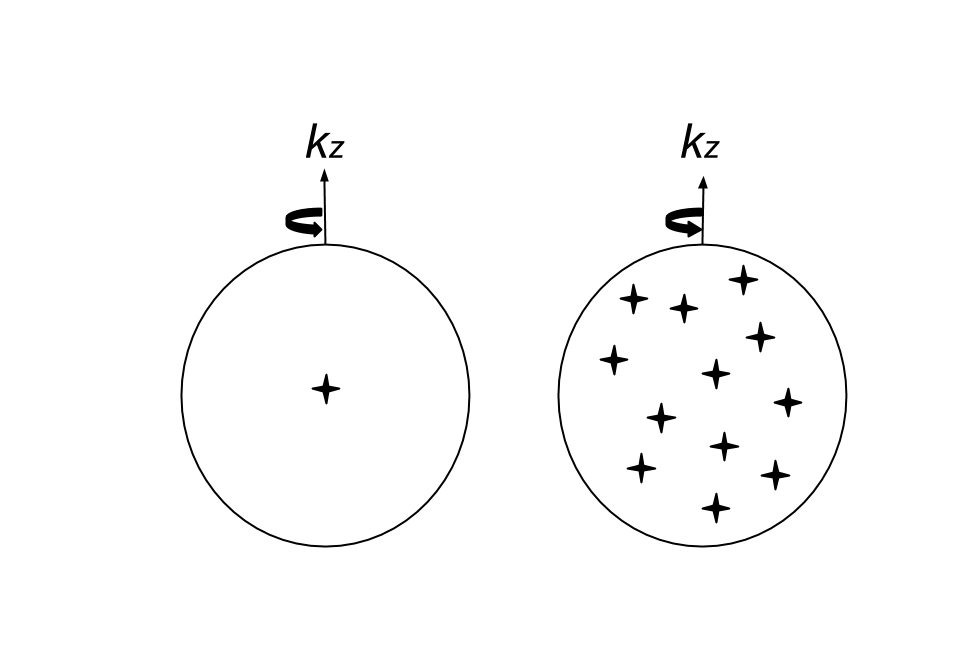
\includegraphics[scale=0.3]{Figures/models.png}
\end{figure}
\end{frame}


\begin{frame}{\textit{\textbf{Models:}}}
\begin{table}
\begin{center}
\begin{tabular}{llc}\hline\hline
Physical Parameter (units) & Symbol & Values\\\hline
Velocity ($km/s$) & $V_{\rm max}$&$0,\ \ 100,\ 200,\ 300$\\
Hydrogen Optical Depth & $\tau_{H} $ & $10^{5},\ 10^{6},\ 10^{7}$\\
Dust Optical Depth & $\tau_{a}$ & $0$,$1$\\
Photons Distributions & & Central, Homogeneous\\\hline\hline
\end{tabular}
\caption{Summary of Physical Parameters of our Monte Carlo Simulations.}
\end{center}
\end{table}
\end{frame}


\begin{frame}{\textit{\textbf{Rotation has an effect on the morphology of the line:}}}
\LARGE{We measure the impact of rotation and viewing angle $\theta$ for the 
main line characteristics.}
\begin{figure}
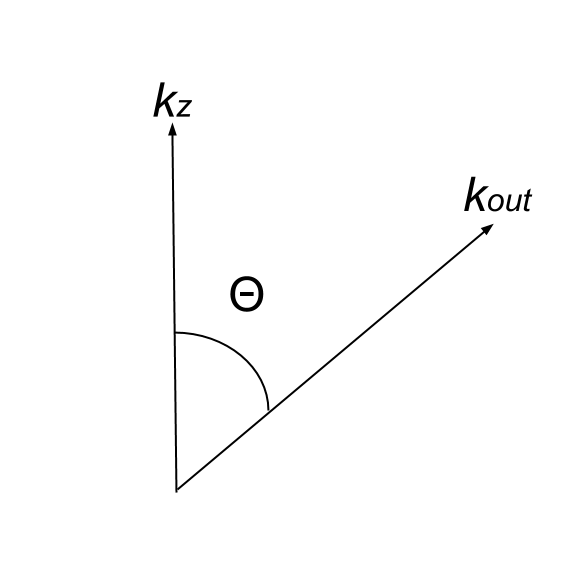
\includegraphics[scale=0.2]{Figures/theta.png}
\end{figure}
\end{frame}

\begin{frame}{\textit{\textbf{The morphology of the line is affected by rotation}}}
\begin{figure}
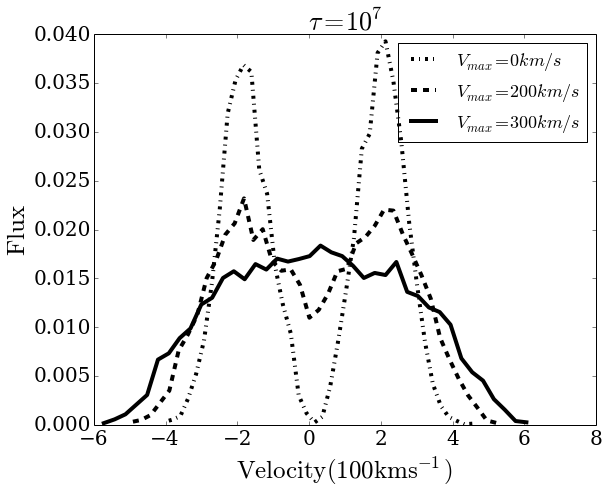
\includegraphics[scale=0.4]{Figures/difvel.png}
\caption*{Garavito-Camargo e.a 2014}
\end{figure}
\end{frame}

\begin{frame}{\textit{\textbf{The morphology of the line changes for different observers}}}
\begin{figure}
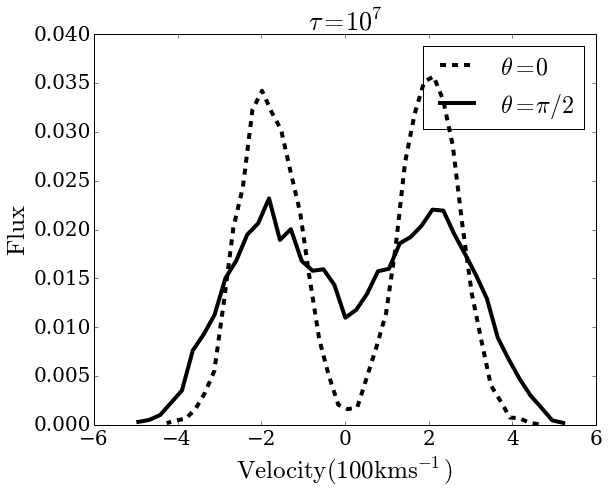
\includegraphics[scale=0.4]{Figures/diftheta.png}
\caption*{Garavito-Camargo e.a 2014}
\end{figure}
\end{frame}


%\begin{frame}{Simulated spectra}
%\begin{figure}
%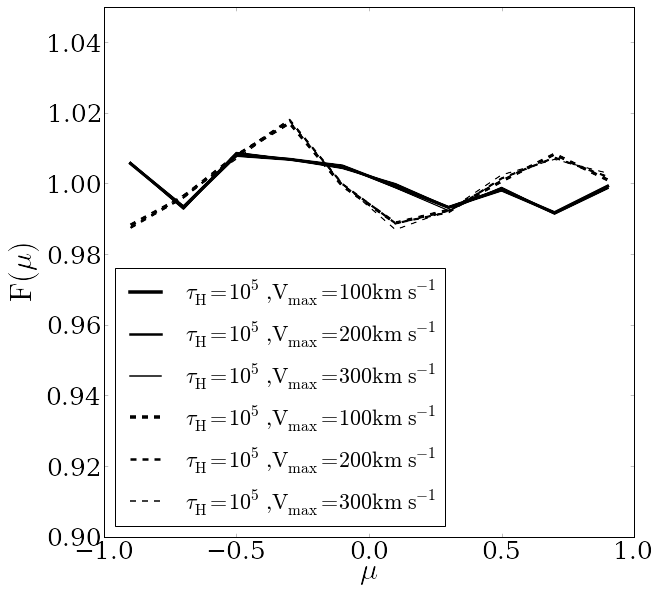
\includegraphics[scale=0.4]{Figures/f5.png}
%\end{figure}
%\end{frame}


\begin{frame}{\textit{\textbf{The line width increases proportional to the rotation velocity.}}}
\begin{figure}
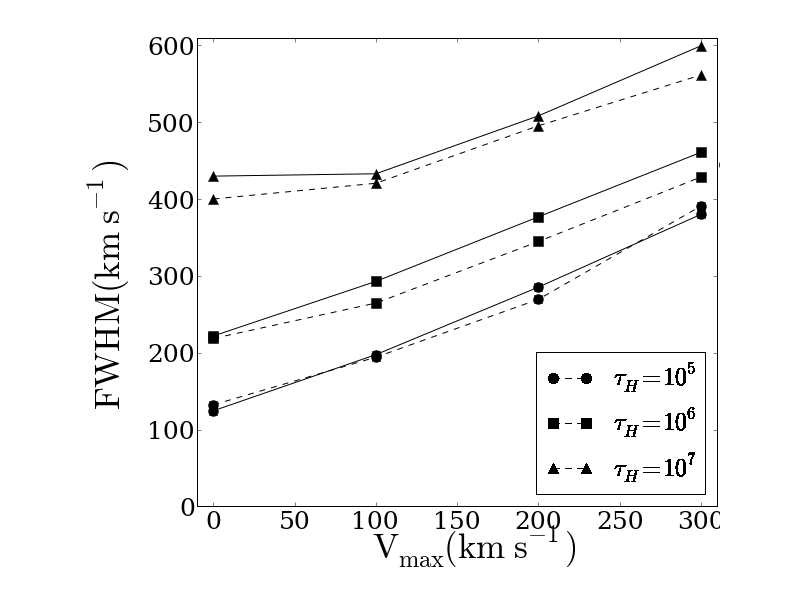
\includegraphics[scale=0.30]{Figures/f71.png}
\caption*{Garavito-Camargo e.a 2014}
\end{figure}
\end{frame}



\begin{frame}{\textit{\textbf{The line width increases proportional to the rotation velocity.}}}
\begin{figure}
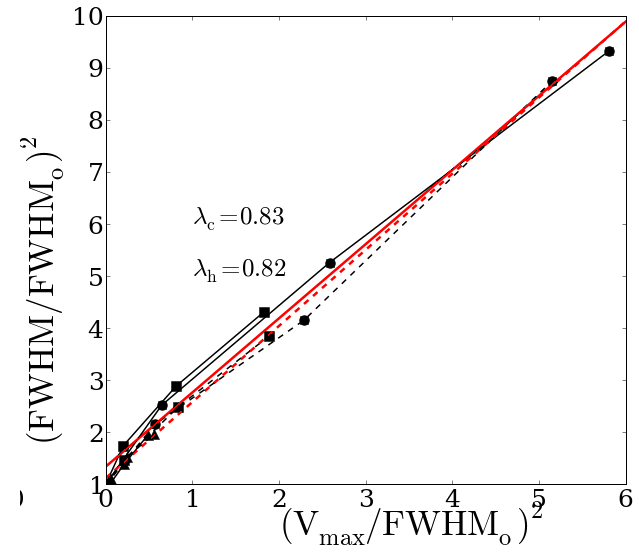
\includegraphics[scale=0.25]{Figures/f72.png}
\caption*{Garavito-Camargo e.a 2014}
\[
FWHM^2 = FWHM_0 ^2 + \left (\dfrac{V_{max}}{\lambda}\right ) ^2
\]

\end{figure}
\end{frame}


\begin{frame}{\textit{\textbf{The line width increases proportional to the viewing angle $\theta$}}}
\begin{figure}
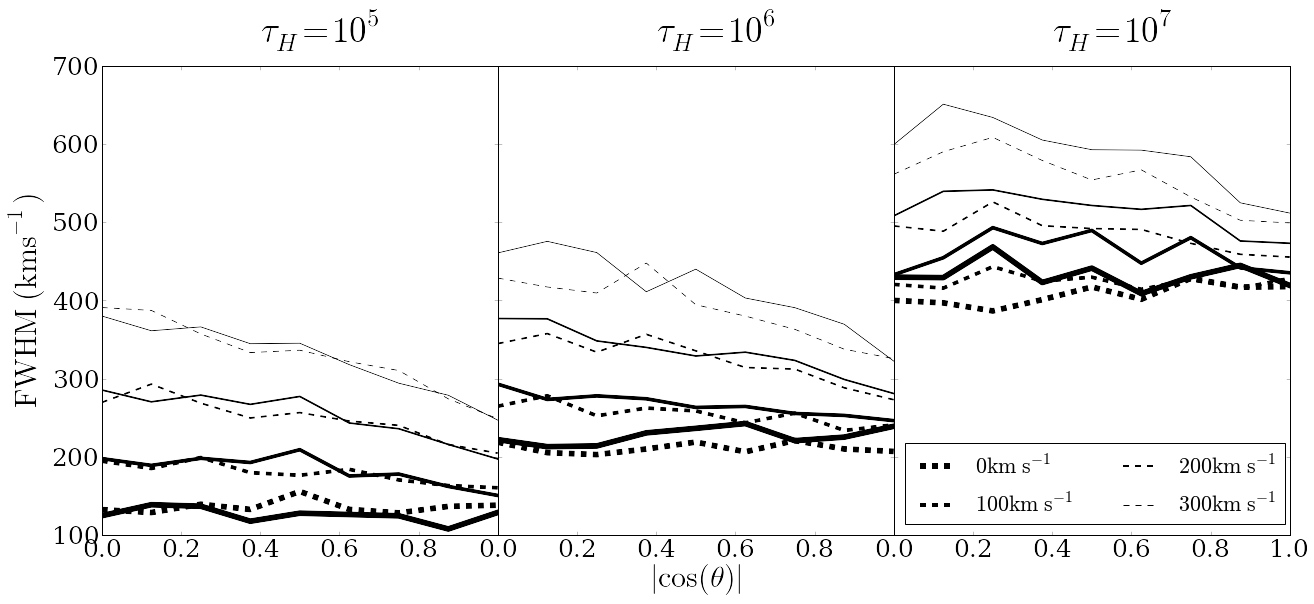
\includegraphics[scale=0.4]{Figures/f6.png}
\caption*{Garavito-Camargo e.a 2014}
\end{figure}
\end{frame}

\begin{frame}{\textit{\textbf{The flux at the line center increases with the rotation velocity and the viewing angle $\theta$.}}}
\begin{figure}
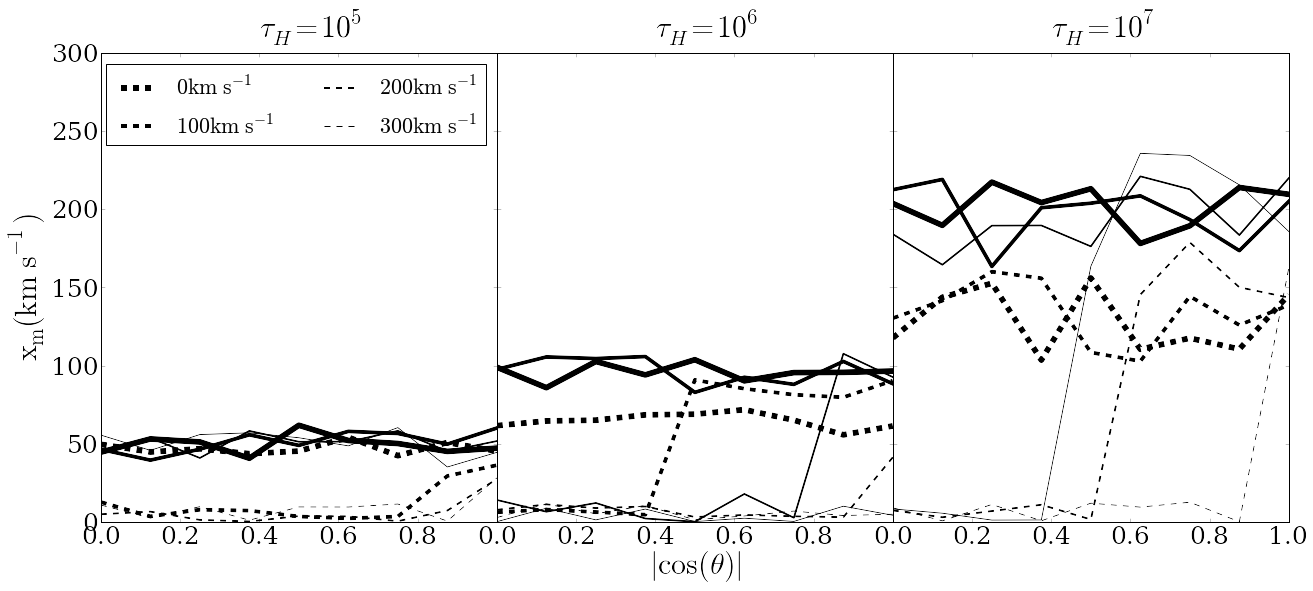
\includegraphics[scale=0.4]{Figures/f8.png}
\caption*{Equator \ \ \ \ \ \ \    Garavito-Camargo e.a 2014  \ \ \ \ \ \ Poles}
\end{figure}
\end{frame}

\begin{frame}{\textit{\textbf{The average number of scatterings is unaffected by rotation and viewing angle.}}}
\begin{figure}
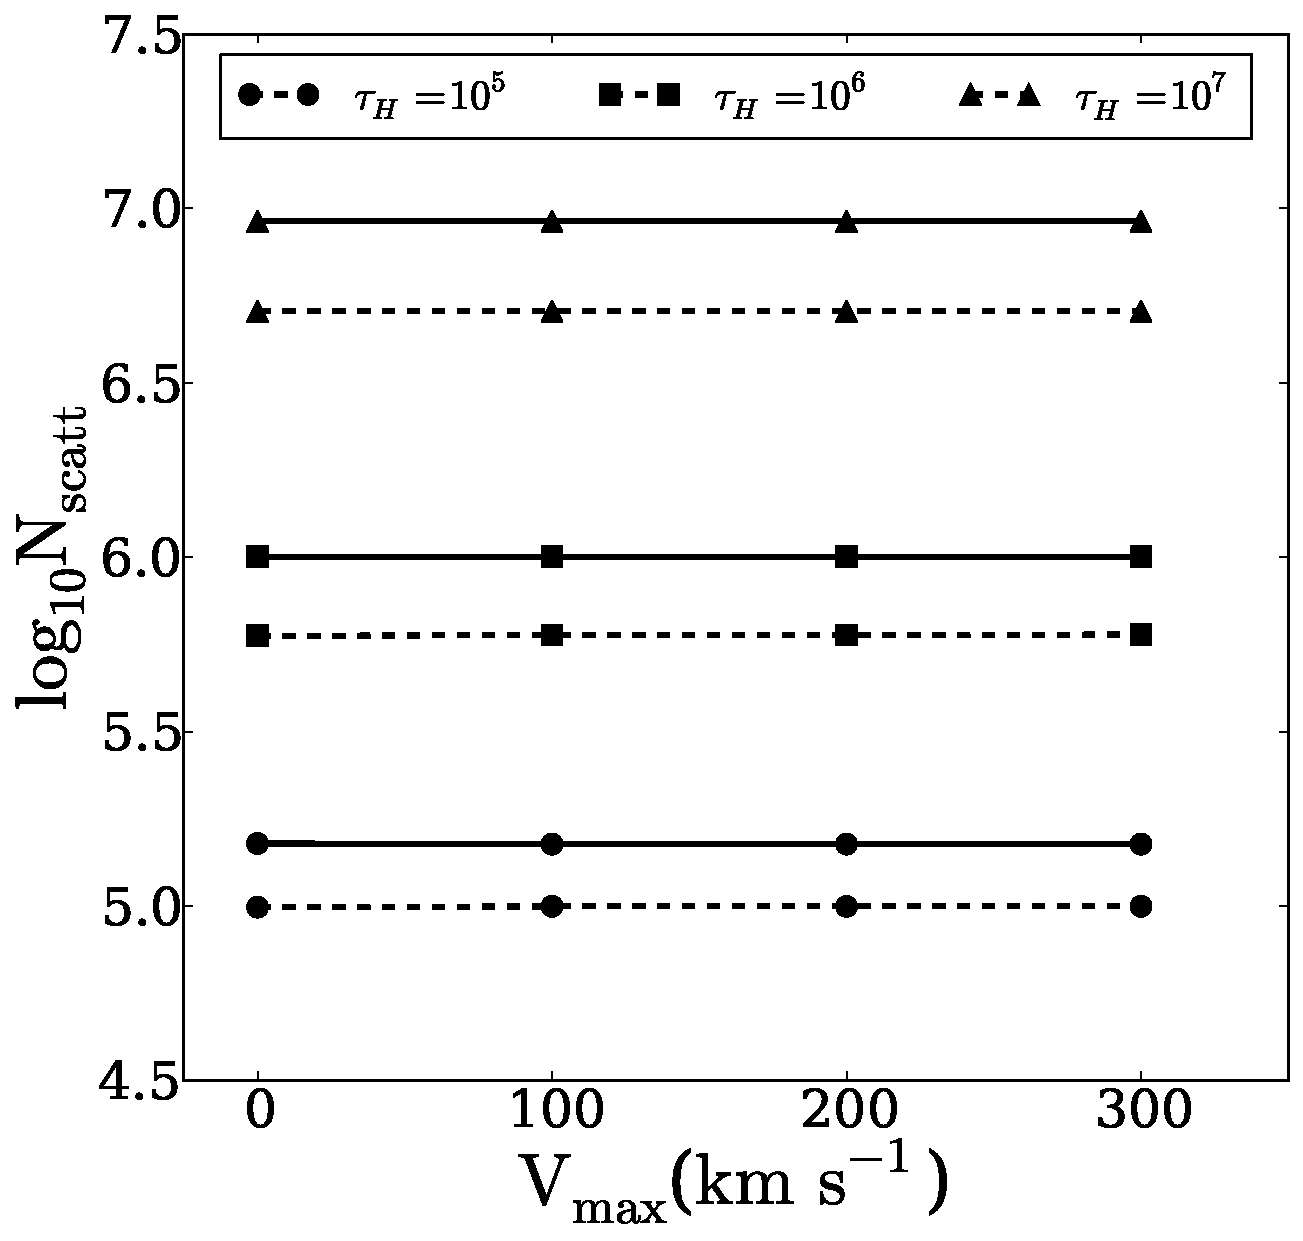
\includegraphics[scale=0.32]{Figures/f13.pdf}
%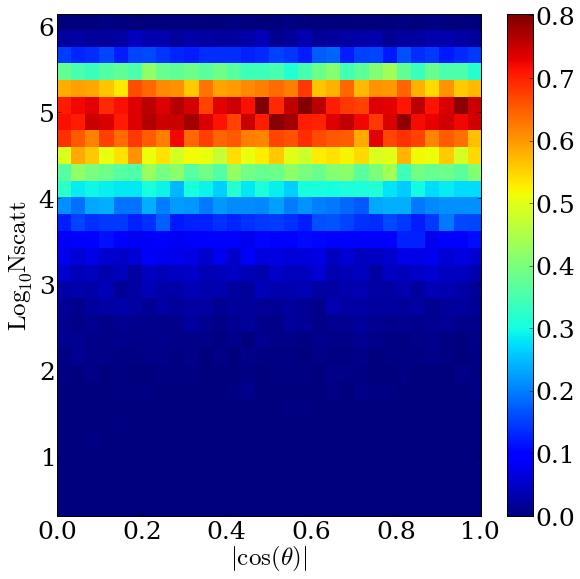
\includegraphics[scale=0.25]{Figures/f9h.png}
\caption*{Garavito-Camargo e.a 2014}
\end{figure}
\end{frame}

\begin{frame}{\textit{\textbf{The escape fraction of Ly$\alpha$ is unaffected by rotation and viewing angle.}}}
\begin{figure}
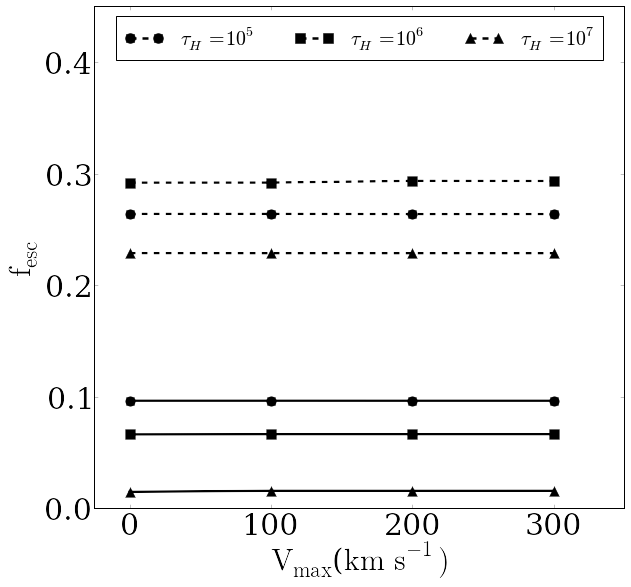
\includegraphics[scale=0.35]{Figures/f10.png}
\caption*{Garavito-Camargo e.a 2014}
\end{figure}
\end{frame}

\begin{frame}{\textit{\textbf{Analytic approximation:}}}
\begin{figure}
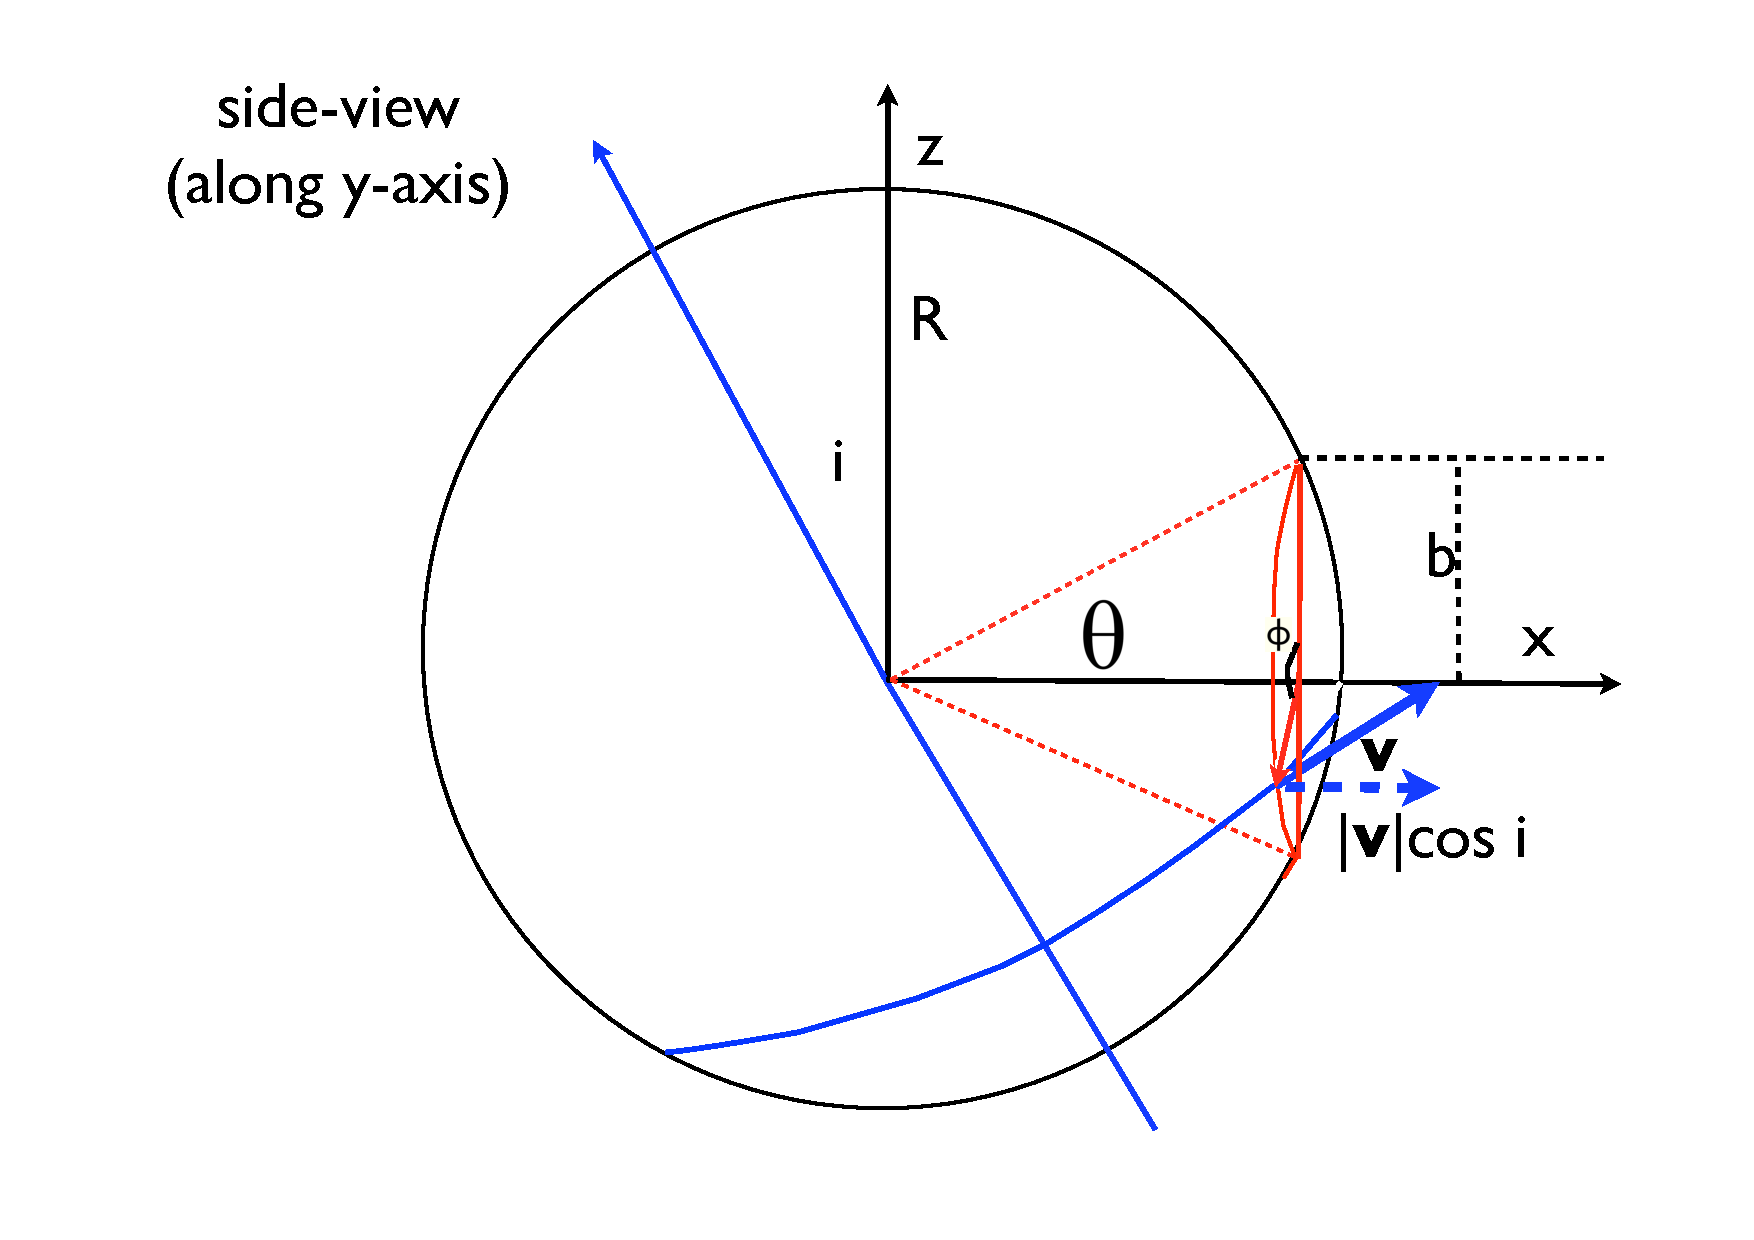
\includegraphics[scale=0.2]{Figures/fig11a.pdf}
\end{figure}
%\begin{equation}
%J(x, b, \phi, i) = \dfrac{\sqrt{\pi}}{\sqrt{24}a\tau}\left( \dfrac{(x - x_b)^2}{1 + cosh[\sqrt{\dfrac{2\pi^3}{27}}\dfrac{|(x-x_b)^3|}{a\tau}]} \right ) 
%\end{equation}


\begin{equation}
J(x, i) = 2\pi \int \limits_0^R db b \int \limits_0^{2\pi}d\phi S(b,\phi)J(x, b, \phi, i) \approx 2\pi \int \limits_0^R db b \int \limits_0^{2\pi}d\phi J(x, b, \phi, i)
\end{equation}
\end{frame}

%\begin{frame}
%\begin{figure}
%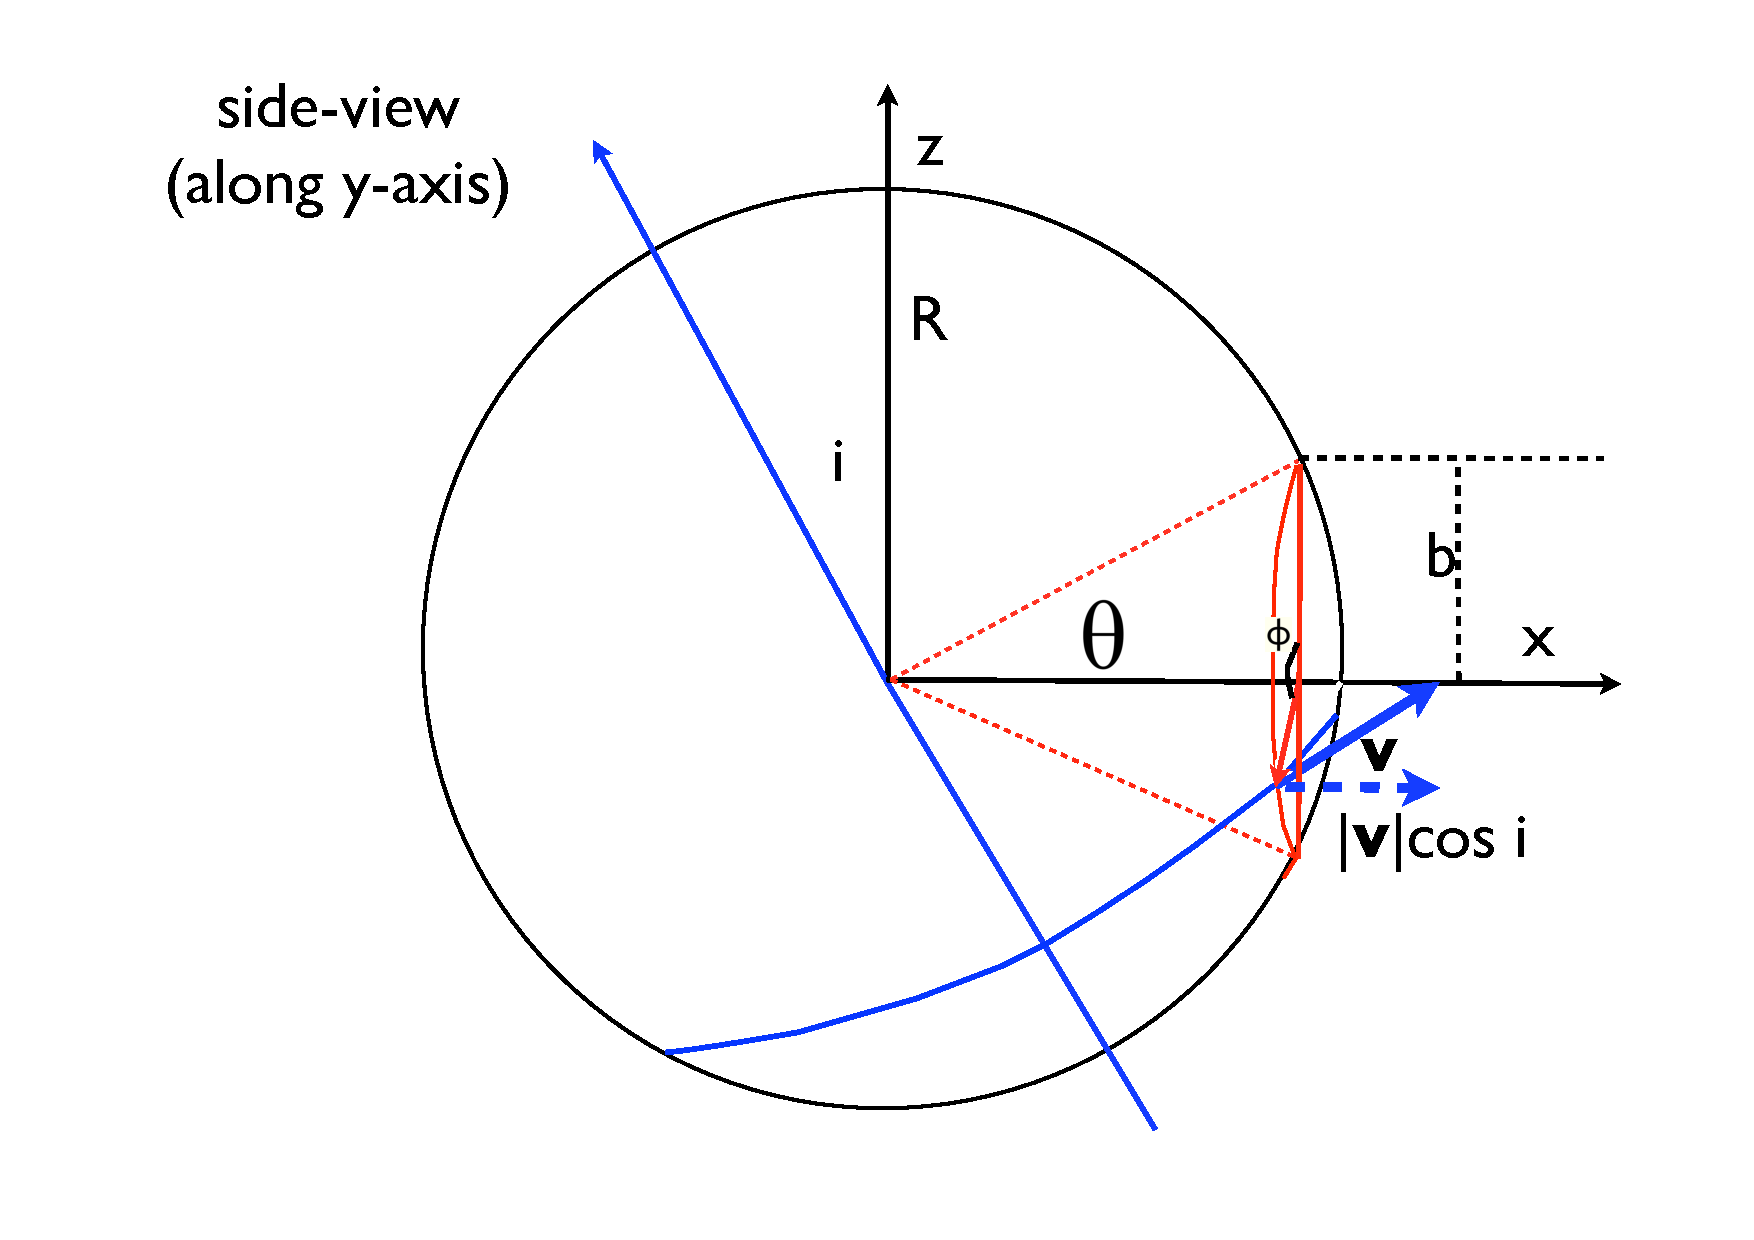
\includegraphics[scale=0.2]{Figures/fig11a.pdf}
%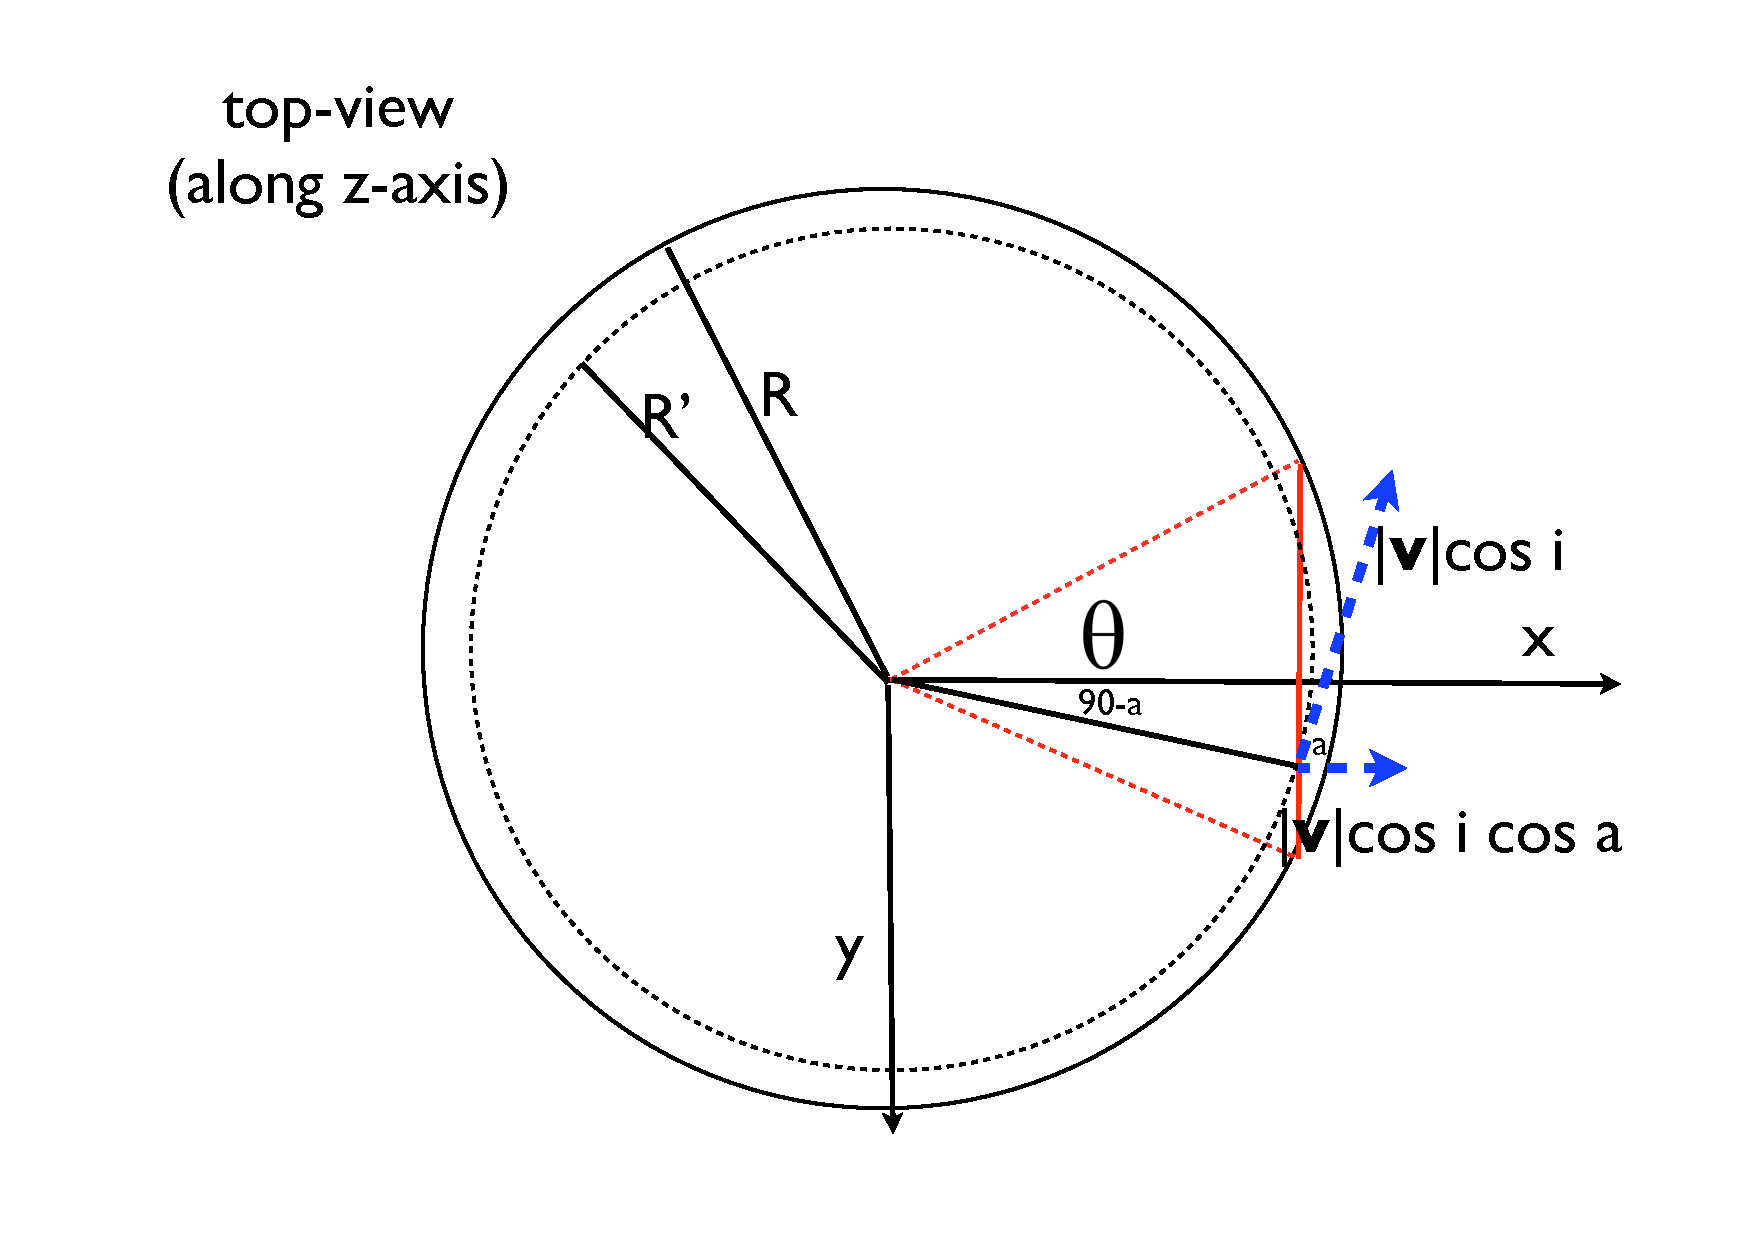
\includegraphics[scale=0.2]{Figures/fig11b.pdf}
%\caption*{Garavito-Camargo e.a 2014}
%\end{figure}

%\begin{equation}
%v_b(b, \phi, i) =   V_{max}\dfrac{\sqrt{R^2 - s^2}}{R}cosi cosa
%\end{equation}

%\begin{equation}
%tan \beta = tan|90^o-a| = \dfrac{c}{d} = \dfrac{b sin \phi}{\sqrt{R^2 - b^2}}
%\end{equation}
%\end{frame}

\begin{frame}{\textit{\textbf{Analytic approximation:}}}
\begin{figure}
%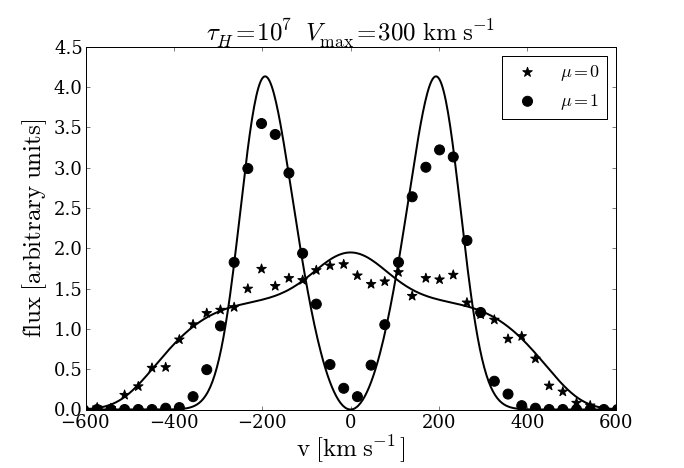
\includegraphics[scale=0.2]{Figures/vary_angle1.png}
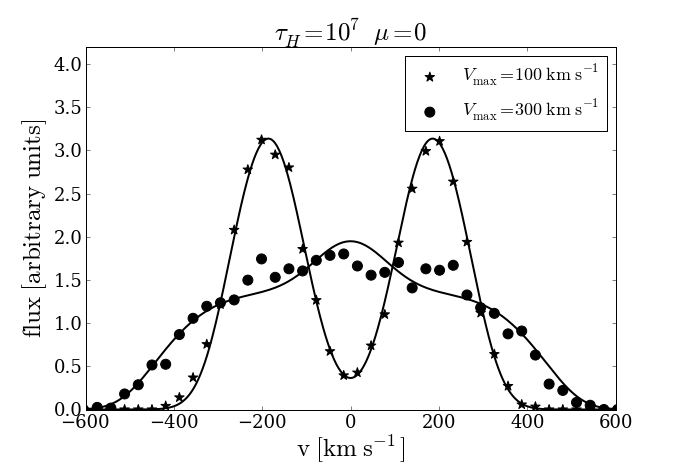
\includegraphics[scale=0.4]{Figures/vary_vel1.png}
\caption*{Garavito-Camargo e.a 2014}
\end{figure}
\end{frame}



\begin{frame}{\textit{\textbf{Lyman alpha observed in rotation:}}}
\begin{figure}
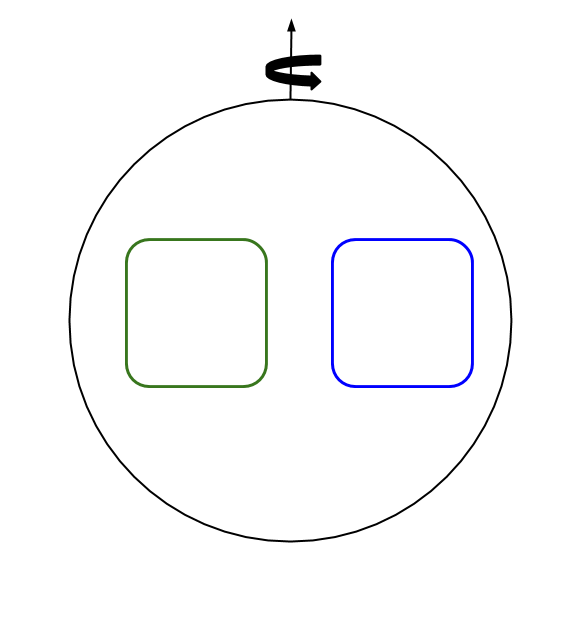
\includegraphics[scale=0.2]{Figures/measure.png}
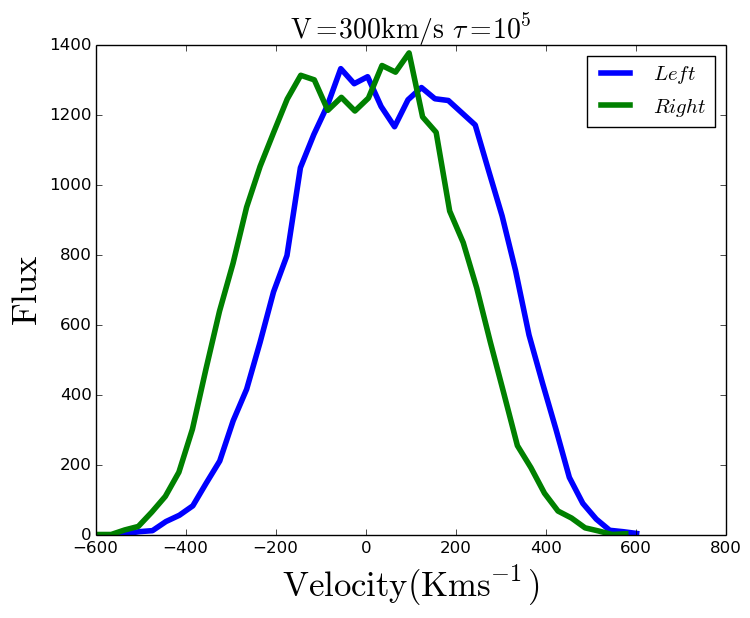
\includegraphics[scale=0.3]{Figures/obs.png}
%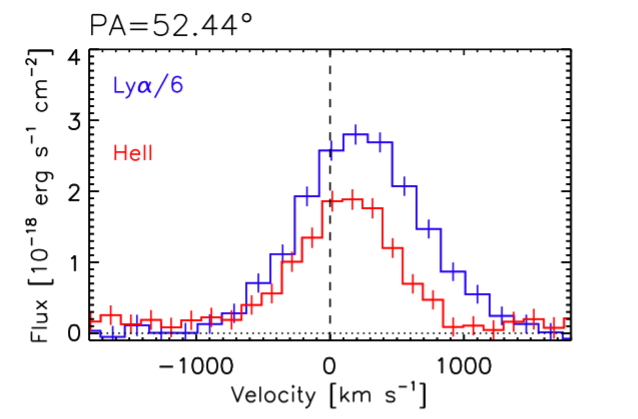
\includegraphics[scale=0.15]{Figures/rotation1.png}
%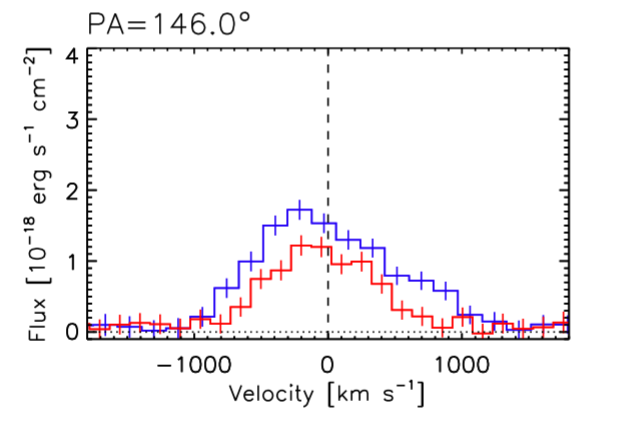
\includegraphics[scale=0.15]{Figures/rotation2.png}
\end{figure}
\end{frame}


\begin{frame}
\begin{figure}
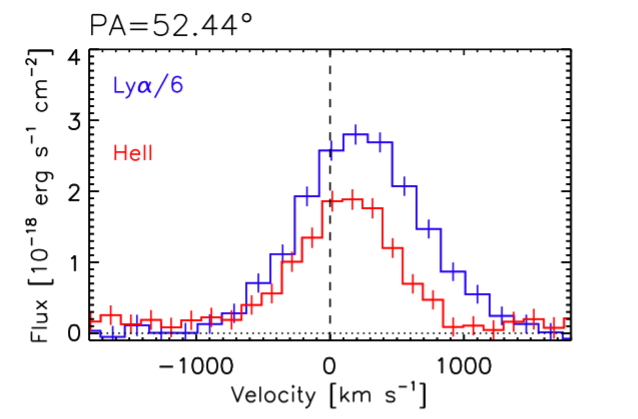
\includegraphics[scale=0.25]{Figures/rotation1.png}
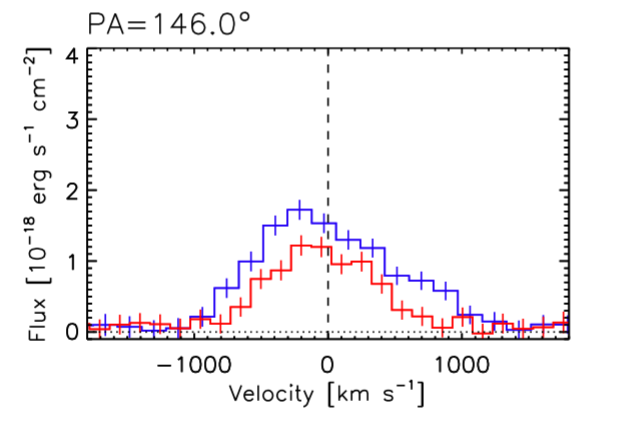
\includegraphics[scale=0.25]{Figures/rotation2.png}
\caption*{Prescott e.a, ApJ,  2014.}
\end{figure}
\end{frame}

\begin{frame}{\textit{\textbf{Conclusions:}}}
\textbf{1.} Rotation has an impact in the Ly$\alpha$ line morphology; the width and the relative intensity of the peaks and the center of the line are affected.
\[
FWHM^2 = FWHM_0^2 + \left( \dfrac{V_{max}}{\lambda} \right )^2
\]

\begin{figure}
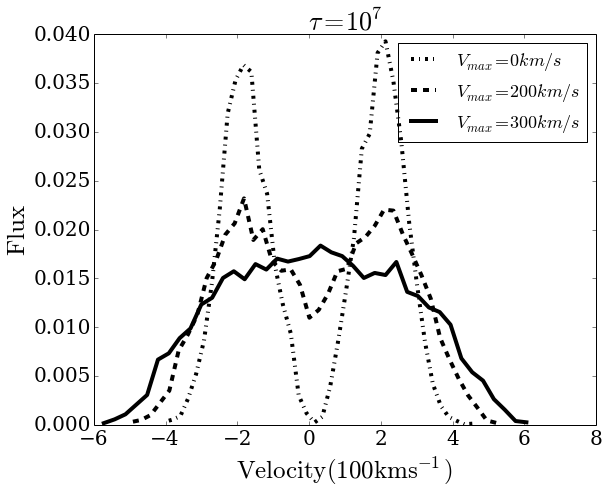
\includegraphics[scale=0.3]{Figures/difvel.png}
\end{figure}

\end{frame}

\begin{frame}{\textit{\textbf{Conclusions:}}}
\textbf{2.} Rotation induces an anisotropy for different viewing angles.
\begin{figure}
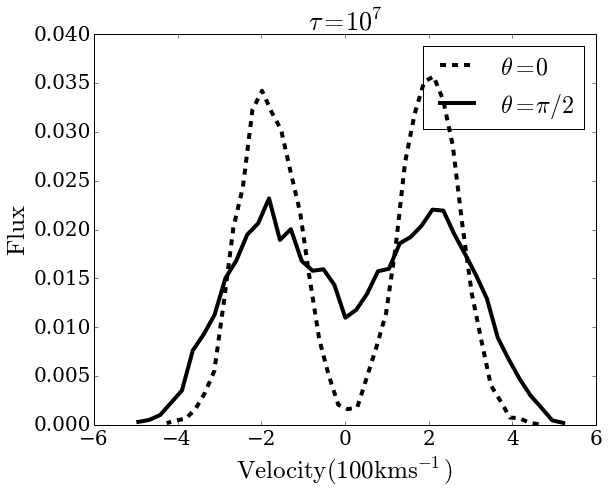
\includegraphics[scale=0.3]{Figures/diftheta.png}
\end{figure}
\end{frame}


\begin{frame}{\textit{\textbf{Conclusions:}}}
\textbf{3.} An analytical approximation could be derived.
\begin{figure}
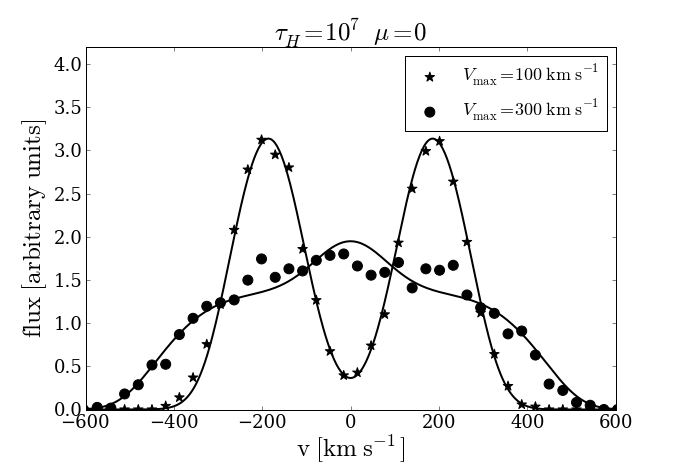
\includegraphics[scale=0.3]{Figures/vary_vel1.png}
\end{figure}
\end{frame}

\begin{frame}{\textit{\textbf{In progress:}}}
\begin{figure}
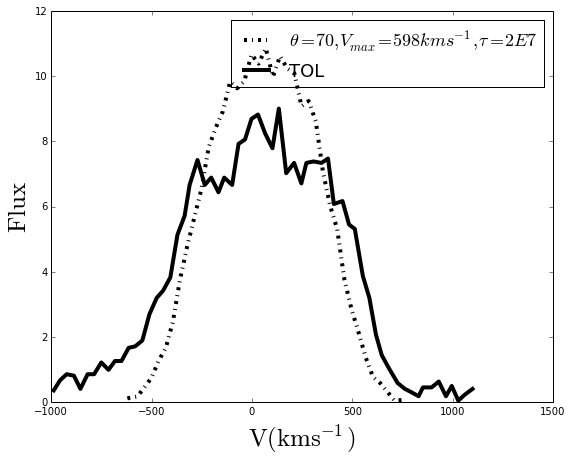
\includegraphics[scale=0.4]{Figures/CLARA-TOL.png}
\end{figure}
\end{frame}

%\begin{frame}{Work in progress}
%rotation + outfloes
%\end{frame}

\end{document}
